\chapter{Matlab Simulation}

We implemented a MATLAB simulation of the robot using the Robotics Toolbox. This toolbox is capable of calculating robot trajectories, calculate inverse kinematics, visualize the simulated system etc. The MATLAB model is based on the kinematics and dynamics models obtained from 
\todo{reference the articles}. The simulation shows the end effector's reaction to arbitrary input and is able to calculate the time needed to reach the goal with the given input signals.

\begin{figure}[H]
	\centering
	\begin{subfigure}{.32\textwidth}
		\centering
		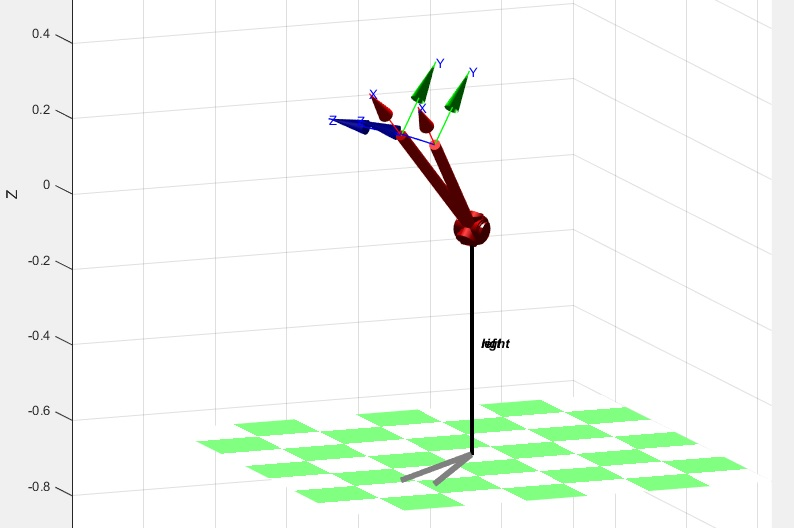
\includegraphics[width=\linewidth]{matlab_sim.jpg}
		\caption{Visual representation of the simulation \vspace{8.5mm}   }
		\label{fig:matlab_sim}
	\end{subfigure}
\end{figure}


